\documentclass[12pt]{article}
\usepackage{graphicx}

\oddsidemargin  -0.5 cm
\evensidemargin 0.0 cm
\textwidth      6.5in
\headheight     0.0in
\topmargin      -1 cm
\textheight=9.0in

\title{Di-electron Widths of $\Upsilon(1S)$, $\Upsilon(2S)$, $\Upsilon(3S)$ Update}
\author{Jim Pivarski}

\begin{document}

\maketitle

\setcounter{section}{-1}
\section{Introduction}

This document is a {\it list} of differences between the
EPS/Lattice05/PANIC05 preliminary $\Gamma_{ee}$ result and the final
PRL result up for vote on December 3.

\section{Efficiency Determination}

\subsection{``Visible to Trigger'' Part}

The top of Table I, page 10, presents the probability that an
$\Upsilon(1S)$ hadronic decay will generate at least one trigger track
and at least one CBLO cluster (it is ``visible''), determined from fit
yields to $\pi^+\pi^-$ recoil mass from $\Upsilon(2S) \to \pi^+\pi^-
\Upsilon(1S)$ decays captured by the TwoTrack trigger (see text).
This inferred probability is consistent with 100\%, and must be
corrected for the part of its probability distribution that is greater
than 100\%.  Because the $\Upsilon(1S)$ events include leptonic
decays, and these have a different (greater) probability of being
``invisible,'' we must use the Monte Carlo simulation to correct for
this.  The first correction was applied incorrectly and the second was
omitted in the preliminary results.  Applying both correctly changes
this number from (99.45 $^{+0.34}_{-0.32}$)\% to (99.59
$^{+0.29}_{-0.45}$)\%.

\subsection{``Cascade to Leptons'' Correction}

In Table II, page 14, the lines labeled ``$\Upsilon(2S)$,
$\Upsilon(3S)$ cascade to leptons branching fraction'' have been
recalcuated with more data and a different technique.  The same
criteria were applied to select decays containing $\Upsilon \to
\mu^+\mu^-$, but instead of using a small subset of the $\Upsilon(2S)$
and $\Upsilon(3S)$ data (about a dozen runs), we use the entire
$\Upsilon(2S)$ and $\Upsilon(3S)$ datasets, and the continuum
subtraction is now derived from the lineshape fit results.

To determine the branching fraction of $\Upsilon(2,3S) \to X
\mu^+\mu^-$, we now fit the invariant mass spectrum to a Monte Carlo
simulation, as shown in Figure \ref{beaut}.  Only the magnitudes of
$\Upsilon(2,3S) \to X \mu^+\mu^-$ and $\Upsilon(2,3S) \to \mu^+\mu^-$
are allowed to float: the branching fraction of $X \mu^+\mu^-$ is
measured relative to known $\mu^+\mu^-$ branching fractions, with a
10\% uncertainty assigned for the fitting technique.

\begin{figure}
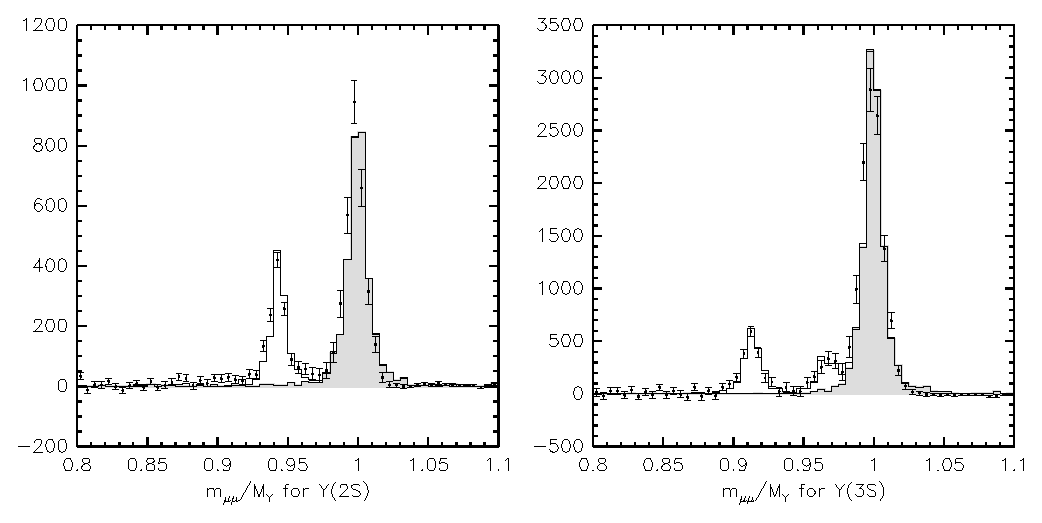
\includegraphics[width=\linewidth]{/home/mccann/monster_talk/beautiful_bcasll_2}
\caption{\label{beaut} Invariant mass of muon pairs (divided by $\Upsilon$ mass) for $\Upsilon(2S)$ and $\Upsilon(3S)$.  Points are data, histograms are Monte Carlo simulations, and shaded area is prompt $\Upsilon \to \mu^+\mu^-$.}
\end{figure}

The old values for the branching fractions, (1.54 $\pm$ 0.36)\% and
(1.44 $\pm$ 0.48)\%, are now (1.58 $\pm$ 0.16)\% and (1.34 $\pm$
0.13)\%, respectively.

\section{Point-to-Point Luminosity is Now from Bhabhas}

While the preliminary results used $e^+e^- \to \gamma\gamma$ events to
determine the luminosity of each point in the scan (and Bhabhas,
$e^+e^- \to \mu^+\mu^-$, and $e^+e^- \to \gamma\gamma$ to determine
the overall scale), the final results use Bhabhas to determine the
luminosity of each point in the scan.  This improves the statistical
precision by a factor of 2.2, which is especially helpful for
determining ratios of $\Gamma_{ee}$, which are statistically limited.

This introduces contamination from $\Upsilon \to e^+e^-$, which is
readily calculated from the total $\Upsilon$ cross-section, from the
lineshape fit.  At a given center-of-mass energy $E$, the number of
$\Upsilon \to e^+e^-$ contaminating the Bhabha count is
\begin{equation}
\sigma(E) {\mathcal B}_{ee} \frac{\int_{-0.76}^{0.76} \cos^2\theta \,
  d\cos\theta}{\int_{-1}^{1} \cos^2\theta \, d\cos\theta} {\mathcal L}(E)
\end{equation}
where $\sigma(E)$ is the $\Upsilon$ production cross-section
(determined from the fit result by a quickly-converging iterative
process), ${\mathcal B}_{ee}$ is the $e^+e^-$ branching fraction (we
assume ${\mathcal B}_{ee}$ = ${\mathcal B}_{\mu\mu}$), and ${\mathcal
  L}(E)$ is the integrated luminosity of the point (determined from
$\gamma\gamma$).  For the $\Upsilon(1S)$, $\Upsilon(2S)$, and
$\Upsilon(3S)$, this is a 5\%, 2\%, and 2\% correction at the peak,
respectively.

Because we calculate $\sigma(E)$ with our standard fit function, we
can easily add the interference term once we know the effective Bhabha
cross-section.  This term is smaller than the direct $\Upsilon \to
e^+e^-$ contamination and negligibly affects the fitted $\Gamma_{ee}$.

\subsection{Now Sensitive to Variations in Beam Energy Spread}

With this new statistical sensitivity, the tall, narrow $\Upsilon(1S)$
peak is now sensitive to 1\% variations in beam energy spread.
Between March 15 and April 7, 2002, the CESR beam energy spread
narrowed by 1.5--1.9\%.  (See my September 2005 PTA talk for plots.)

This change in beam energy spread was coincident with large changes in
the CESR horizontal steerings, and CESRV simulations confirmed that
large changes in the electron orbit, corrected by changes in the
horizontal steerings, yield a 1\% beam energy spread difference.  We
therefore identified all large changes in horizontal steerings as
potential shifts in beam energy spread and fitted the data between
them with different beam energy spread values.  Every $\Upsilon(3S)$
scan, therefore, has a different beam energy spread parameter, the
$\Upsilon(1S)$ has three: Jan 16 -- Feb 20 (2002), Feb 27 -- Mar 13,
and Apr 8 -- Apr 10, and the $\Upsilon(2S)$ has a constant beam energy
spread for all scans.

\subsection{Now Sensitive to Magnitude of Interference Term}

In both the preliminary result and the final result, we assume that
only $\Upsilon \to q\bar{q}$ interferes with the hadronic continuum.
It is conceivable that $\Upsilon \to ggg
$ would as well, if the
``$\Upsilon \to$ intermediate state $\to$ hadronic final state'' process
does not factorize.  (The third intermediate state, $gg\gamma$, has a
distinct high-energy photon and a much smaller rate than $q\bar{q}$
and $ggg$.)  With the additional statistical power, we tested this
assumption on the $\Upsilon(1S)$.  We effectively fit for the
magnitude of the interference term $y_{int}$ by fitting with different
$y_{int}$ hypotheses, shown in Figure \ref{intscan}.  The fit prefers
a $y_{int}$ of 0.0163 $\pm$ 0.0044, consistent with $q\bar{q}$-only
interference and inconsistent with $|q\bar{q}| + |ggg|$ interference.  The
fraction of $\Upsilon$ decays $f$ participating in continuum interference
is related to $y_{int}$ by $y_{int} \propto \sqrt{f}$, so this
fraction is determined to 13\% of itself.  Varying $y_{int}$ by its
uncertainty alters $\Gamma_{ee}$ by 0.2\%.

\begin{figure}
\includegraphics[width=\linewidth]{/home/mccann/antithesis/interferencescan}
\caption{\label{intscan} Best-fit $\chi^2$ for $\Upsilon(1S)$ fits
  with different interference term magnitudes $y_{int}$ (points) and a
  parabola drawn through them (line).  If only $\Upsilon \to q\bar{q}$
  interferes with continuum hadrons, $y_{int}$ = 0.0174 (circled
  point), and if all hadronic $\Upsilon$ decays interfere with
  continuum hadrons, $y_{int}$ = 0.0560.  Dashed and dotted vertical
  lines indicate the minimum and $+1$ intervals of $y_{int}$.}
\end{figure}

\subsection{Still Insensitive to the Full Width}

Our fits are still insensitive to the $\Upsilon$ full width $\Gamma$,
and its effect on the fitted value of $\Gamma_{ee}$ is still
negligible.

\section{Dropped April 3 Scan}

The April 3 scan, included in the preliminary result, is dropped in
the final result.  This scan contains measurements on one side of the
peak only and cannot be joined with a more complete scan.  This
omission reduces $\chi^2$ by 32 (out of 187 constraints) but changes
$\Gamma_{ee}$ by only 0.006\%.

\section{New Fit Results}

\newcommand{\us}{$\Upsilon(1S)$}
\newcommand{\uss}{$\Upsilon(2S)$}
\newcommand{\usss}{$\Upsilon(3S)$}
\newcommand{\chired}{\chi^2_{\mbox{\scriptsize red}}}

The results are plotted in Figure \ref{fits}.  The reduced $\chi^2$,
or $\chi^2/($number of points $-$ degrees of freedom$)$ for \us\ is
$240/(203-16) = 1.3$ (0.5\% C.L.), for \uss\ is $107.2/(75-9) = 1.6$
(0.1\% C.L.), and for \usss\ is $155/(175-16) = 0.97$ (59\% C.L.).
Pull distributions versus energy and versus date (Figures
\ref{pulls1}, \ref{pulls2}, and \ref{pulls3}) show no obvious trends.
(See PRL draft for more discussion.)

\begin{figure}
\begin{center}
\includegraphics[width=0.8\linewidth]{/home/mccann/antithesis/fit_results/novemberfits_noapr03_3_10_final_allfit_comb3}
\end{center}
\caption{\label{fits} Lineshape fits for (a) $\Upsilon(1S)$, (b) $\Upsilon(2S)$, and (c) $\Upsilon(3S)$.  Vertical axis should be ``Selected events / nb$^{-1}$,'' as data (points) are not corrected for efficiency and contain a flat background contamination from radiative Bhabhas (about half of the continuum).  The solid line is the best fit and the dashed line is the sum of all backgrounds.  Insets enlarge the high-energy tail point they are placed over.  Points within 1 MeV of each other are combined in the plot, but not in the fit.}
\end{figure}

\begin{figure}
\begin{center}
\includegraphics[width=0.8\linewidth]{/home/mccann/antithesis/fit_results/novemberfits_noapr03_3_10_pulls1again}
\end{center}
\caption{\label{pulls1} Pulls (fit residual divided by uncertainty) versus (a) energy, (b) date, and (c) as a histogram for the $\Upsilon(1S)$.  No points have been combined; this is what was used in the fit.}
\end{figure}

\begin{figure}
\begin{center}
\includegraphics[width=0.8\linewidth]{/home/mccann/antithesis/fit_results/novemberfits_noapr03_3_10_pulls2again}
\end{center}
\caption{\label{pulls2} Pulls (fit residual divided by uncertainty) versus (a) energy, (b) date, and (c) as a histogram for the $\Upsilon(2S)$.  No points have been combined; this is what was used in the fit.}
\end{figure}

\begin{figure}
\begin{center}
\includegraphics[width=0.8\linewidth]{/home/mccann/antithesis/fit_results/novemberfits_noapr03_3_10_pulls3again}
\end{center}
\caption{\label{pulls3} Pulls (fit residual divided by uncertainty) versus (a) energy, (b) date, and (c) as a histogram for the $\Upsilon(3S)$.  No points have been combined; this is what was used in the fit.}
\end{figure}

\end{document}
